%  ========================================================================
%  Copyright (c) 1985 The University of Washington
%
%  Licensed under the Apache License, Version 2.0 (the "License");
%  you may not use this file except in compliance with the License.
%  You may obtain a copy of the License at
%
%      http://www.apache.org/licenses/LICENSE-2.0
%
%  Unless required by applicable law or agreed to in writing, software
%  distributed under the License is distributed on an "AS IS" BASIS,
%  WITHOUT WARRANTIES OR CONDITIONS OF ANY KIND, either express or implied.
%  See the License for the specific language governing permissions and
%  limitations under the License.
%  ========================================================================
%

% Documentation for University of Washington thesis LaTeX document class
% by Jim Fox
% fox@washington.edu
%
%    Revised 2020/02/24, added \caption()[]{} option.  No ToC.
%
%    Revised for version 2015/03/03 of uwthesis.cls
%    Revised, 2016/11/22, for cleanup of sample copyright and title pages
%
%    This document is contained in a single file ONLY because
%    I wanted to be able to distribute it easily.  A real thesis ought
%    to be contained on many files (e.g., one for each chapter, at least).
%
%    To help you identify the files and sections in this large file
%    I use the string '==========' to identify new files.
%
%    To help you ignore the unusual things I do with this sample document
%    I try to use the notation
%       
%    % --- sample stuff only -----
%    special stuff for my document, but you don't need it in your thesis
%    % --- end-of-sample-stuff ---


%    Printed in twoside style now that that's allowed
%
 
\documentclass [11pt, proquest] {uwthesis}[2020/02/24]
 
%
% The following line would print the thesis in a postscript font 

% \usepackage{natbib}
% \def\bibpreamble{\protect\addcontentsline{toc}{chapter}{Bibliography}}

\setcounter{tocdepth}{1}  % Print the chapter and sections to the toc
 

% ==========   Local defs and mods
%

% --- sample stuff only -----
% These format the sample code in this document

\usepackage{alltt}  % 
\newenvironment{demo}
  {\begin{alltt}\leftskip3em
     \def\\{\ttfamily\char`\\}%
     \def\{{\ttfamily\char`\{}%
     \def\}{\ttfamily\char`\}}}
  {\end{alltt}}
 
% metafont font.  If logo not available, use the second form
%
% \font\mffont=logosl10 scaled\magstep1
\let\mffont=\sf
% --- end-of-sample-stuff ---

% Table 5.1
\usepackage{amsmath}
\usepackage{graphicx}
\usepackage{array}

\begin{document}
 
% ==========   Preliminary pages
%
% ( revised 2012 for electronic submission )
%

\prelimpages
 
%
% ----- copyright and title pages
%
\Title{GhostPeerShare}
\Author{Jeffrey Murray Jr}
\Year{2024}
\Program{Cybersecurity Engineering}

\Chair{Brent Lagesse}{Ph.D}{Computing \& Software Systems}
\Signature{Geethapriya Thamilarasu}
\Signature{Yang Peng}

\copyrightpage

\titlepage  

 
%
% ----- signature and quoteslip are gone
%

%
% ----- abstract
%


\setcounter{page}{-1}
\abstract{%
This sample dissertation is an aid to students who are attempting
to format their theses with \LaTeX, a sophisticated
text formatter widely used by mathematicians and scientists everywhere.
 
\begin{itemize}
\item It describes the use of a specialized
macro package developed specifically for thesis production
at the University.
The macros customize \LaTeX\ for the correct thesis style,
allowing the student to concentrate on the substance of
his or her text.%
\footnote{See Appendix A to obtain the source to this
 thesis and the class file.}
\item It demonstrates the solutions to a variety of
formatting challenges found in thesis production.
\item It serves as a template for a real dissertation.
\end{itemize}
}
 
%
% ----- contents & etc.
%
\tableofcontents
\listoffigures
\listoftables
 
%
% ----- glossary 
%
\chapter*{Glossary}      % starred form omits the `chapter x'
\addcontentsline{toc}{chapter}{Glossary}
\thispagestyle{plain}
%
\begin{glossary}
\item[Fully Homomorphic Encryption (FHE)] A type of encryption that allows computations to be performed on encrypted data without needing to decrypt it, ensuring data privacy throughout the processing.

\item[Cheon-Kim-Kim-Song (CKKS) Scheme] A fully homomorphic encryption scheme that supports approximate arithmetic on real numbers, particularly useful for decimal-based computations.

\item[Microsoft Simple Encrypted Arithmetic Library (SEAL)] An open-source library developed by Microsoft for implementing homomorphic encryption, supporting arithmetic operations on encrypted data.

\item[Kullback-Leibler Divergence (KLD)] A measure of how one probability distribution diverges from a second, reference probability distribution, used in similarity analysis.

\item[Bhattacharyya Coefficient (BC)] A similarity measure that quantifies the amount of overlap between two probability distributions, commonly used in pattern recognition.

\item[Cramer's Distance (CD)] A statistical measure used to quantify dissimilarity between two probability distributions, sensitive to sample size.

\item[Probability Distribution Form (PDF)] A method of representing data where each value indicates the relative frequency of occurrences, used here to represent video frames for similarity analysis.

\item[Cumulative Distribution Form (CDF)] A representation of a probability distribution where each value is the cumulative sum of probabilities up to that point, ensuring the last value is equal to one. Used in similarity analysis for comparing probability distributions.

\item[Flutter] An open-source, cross-platform framework by Google for building natively compiled applications for mobile, web, and desktop from a single codebase.

\item[Dart] A programming language optimized for building fast applications on any platform, used in the development of Flutter apps.

\item[Foreign Function Interface (FFI)] A Dart feature that allows interaction with C libraries, enabling functionalities like encrypted computations within the Dart and Flutter ecosystems.

\item[FFmpeg] A multimedia framework commonly used for video and audio processing, used here for video preprocessing in mobile applications.

\item[OpenCV] An open-source computer vision and machine learning software library that provides tools for image and video processing.

\item[Conan] A dependency management tool used for packaging and managing C++ libraries, facilitating cross-compilation for various platforms.

\item[GitHub Actions] A CI/CD tool that automates tasks such as building, testing, and deploying software, supporting the automation of plugin testing and deployment in this project.

\end{glossary}

 
%
% ----- acknowledgments
%
\acknowledgments{% \vskip2pc
  % {\narrower\noindent
  The author wishes to express sincere appreciation to
  University of Washington, where he has had the opportunity
  to work with the \TeX\ formatting system,
  and to the author of \TeX, Donald Knuth, {\it il miglior fabbro}.
  % \par}
}

%
% end of the preliminary pages

%
% ==========      Text pages
%

\textpages
 
% ========== Chapter 1
 
\chapter {Introduction}
 
\section{Problem Statement}
\label{sec:Problem Statement}
The Microsoft Simple Encrypted Arithmetic Library (SEAL) \cite{sealcrypto} requires significant pre-requisite knowledge in C, C++, Kotlin, and Gradle to compile and embed within mobile applications. These prerequisites have limited the accessibility of SEAL, posing a significant obstacle to the adoption within the mobile community.

\section{Stakeholders}
Microsoft was a pioneer in the Fully Homomorphic Encryption research, leading the development of the Simple Encryption Arithmetic Library, SEAL in 2018. SEAL established a foundation for efficient homomorphic encryption, making it accessible for developers and researchers. The open-source community soon contributed to the field with OpenFHE, a flexible, community-driven project that was initially released in 2020. OpenFHE expands upon the capabilities of SEAL, offering a collaborative platform for researchers and developers interested in advancing encryption technology.

Flutter, a versatile and state-of-the-art framework by Google, as of a 2023 study, captures 46\% of the cross-platform framework market [1]. Recognized for its ability to support high-performance, cross-platform applications, Flutter includes a powerful plugin system with a Foreign Function Interface (FFI). This interface enables seamless integration with C libraries, offering null safety, managed memory, and compatibility across major operating systems, including Android, Linux, macOS, iOS, and Windows.

By leveraging Dart, a more portable programming language, developers and security researchers can interact directly with FHE backend libraries. This integration reduces the complexity of working with SEAL or OpenFHE, allowing developers to rapidly build cross-platform applications with homomorphic encryption capabilities. Furthermore, security researchers can extend the application to support additional C/C++ libraries, broadening the scope of FHE implementations and facilitating wider distribution to end-users.

\section{Contributions}
The Pyfhel library (Ibarrondo and Viand, 2021) provides a native Python interface to SEAL cryptosystems, abstracting core SEAL functionalities for easier use. While Pyfhel supports cross-platform compatibility on Windows, Linux, and macOS, it currently lacks support for mobile platforms like Android and iOS. This project adopts a similar approach, creating a modular interface that supports multiple backend libraries and manages them as Dart plugins.

A key contribution of this work is its modular design, which enables the seamless integration and versioning of different backend libraries through Dart plugins. With the use of CMake configurations, each C library can be synchronized and recompiled as new versions become available, simplifying the update process. Automating these compilations reduces maintenance overhead, ensuring that the libraries remain up-to-date with minimal manual intervention.

To assess both the performance and accuracy of the library, we re-implement the Proof of Presence Share methodology. This method calculates similarity scores between videos without exposing their content, providing strong privacy guarantees. We set up cameras from various angles recording simultaneously and compare the videos for similarity, as well as, perform comparisons against other scenes of the same duration. Using a supervised artificial neural network, we classify the distance measures of KLD, Bhattacharya, and Cramer for training and testing so that the model can differentiate between scenes that are similar and those that are distinct. This classification enables us to accurately evaluate the library's effectiveness in identifying matching scenes while maintaining privacy. By analyzing the model’s accuracy across various similarity scores, we gain insight into the precision and reliability of the library in distinguishing matching scenes without revealing the videos’ content.


% ========== Chapter 2
 
\chapter{Background}

\section{Flutter}
Flutter is a modern, open-source software development kit designed to build stylish and efficient applications for mobile, web, and desktop within a single code base. Flutter is built on top of Dart; an object-oriented language with C-style syntax. Dart includes advanced features out of the box such as garbage collection for memory management, synchronous and asynchronous handlers, null safety, and compile-time data type checking. We selected Flutter for its low development cost and a wide variety of plugins.

The plugin at the root of this project's design, the Foreign Function Interface allows the application to invoke functions from pre-compiled C libraries. Each target platform, specifically Windows, Linux, Android, iOS, and macOS requires different methods to compile, however, the fundamental method of invoking C functions and working with native data structures remains the same across platforms. The plugin is limited to transforming primitive data types, e.g. Booleans, Integers, and Characters, restricting the parameters of native C functions to primitive data types. However, a notable workaround to this problem is passing complex objects by memory address, known as pass by reference, for the underlying C library to access the object stored in this stack. 

To facilitate the networking between peer-to-peer Android devices, QuickShare \cite{samsung_quick_2020} was developed by Samsung as a file-sharing utility application for nearby wireless devices. It leverages Bluetooth to discover nearby wireless devices and optionally uses WiFi to transfer large files between two nodes. QuickShare is accessible through a Flutter plugin that enables users to share data using their device's native sharing capabilities. This allows users to easily send content to other apps, such as social media platforms, messaging apps, or email.

Alternatives such as React Native (with JavaScript) or native development languages with Kotlin (Android) and Swift (iOS) involve different compilation methods. React Native is a popular framework for cross-platform development, comparable to Flutter in plugins and community activity, however, lacks the native support of C interoperability and performance. React Native leverages Kotlin and Swift to configure and compile Android and iOS applications, respectively. This approach carries inherent challenges to developing and testing an application, often requiring additional dependencies to handle trivial maintenance. Flutter aims to streamline the process of building cross-platform applications by unifying the codebase, eliminating the need for separate code for each platform. 

\section{Simple Encrypted Arithmetic Library}
\label{sec:Background SEAL}
To perform computations on encrypted data, this project utilizes Simple Encrypted Arithmetic Library (SEAL) \cite{sealcrypto}, an open-source homomorphic encryption library developed by Microsoft. The library supports limited arithmetic including addition, subtraction, and multiplication to be performed directly on encrypted data without needing to decrypt it. We chose SEAL primarily for its maturity, prevalent adoption in research, and use in Proof of Presence Share \cite{Lagesse2021-PopShare}.

SEAL supports three Fully Homomorphic Encryption (FHE) schemes: Brakerski-Fan-Vercauteren (BFV) \cite{fan2012-bfv}, Brakerski-Gentry-Vaikuntanathan (BGV) \cite{brakerski2012-bgv}, and Cheon-Kim-Kim-Song (CKKS) \cite{Cheon2017-CKKS}. BFV and BGV are integer-based FHE schemes that allow for computations on encrypted integers but differ in their ciphertext structure and noise management techniques. BFV encodes the message with the most significant bits of the ciphertext and accumulates more noise growth for each multiplication circuit. When too much noise accumulates, the ciphertext cannot be decrypted. For simpler computations, BFV offers better performance. BGV encodes the message in the least significant bits and manages noise through modulus switching. This difference in noise management makes BGV suitable for deeper computations with many sequential operations. 

CKKS is specifically designed for scenarios where approximate arithmetic is acceptable, and this trade-off allows for more efficient computations on encrypted real numbers. This scheme is efficient in performing computations, by representing real numbers as complex numbers. The encoding allows for efficient arithmetic operations, specifically addition, multiplication, and subtraction. When decoding, the result is transformed into a meaningful representation of the true value, with some degree of error. 

\section{Distance Measures}

To accurately measure the similarity between videos while preserving privacy, this project utilizes Kullback-Leibler Divergence (KLD), Bhattacharyya Coefficient (BC), and Cramer’s Distance (CD). KLD (Kullback and Leibler 1951) is a non-symmetric measure of the difference between two probability distributions. BC (Bhattacharyya 1946) is a symmetric measure of the overlap between two probability distributions. CD (Cramér 1928) is a symmetric measure of the difference between two probability distributions. Following the work of Pop-Share (Lagesse et al. 2021), which established these measures as effective baselines for video similarity analysis. These three metrics were chosen over other probability distribution algorithms due to their reliance on basic arithmetic for homomorphic computations.


% ========== Chapter 3
 
\chapter{Related Work}

In this chapter, we provide an overview of the current research landscape surrounding Fully Homomorphic Encryption, relevant Video Similarity algorithms, and Proof of Presence Share, which serves as the baseline for our implementation.

\section{Fully Homomorphic Encryption Libraries}

Open-Source Fully Homomorphic Encryption Library, OpenFHE [8], is a state-of-the-art C++ library born from a merger of PALISADE, HElib and HEAAN. OpenFHE supports modern schemes and can be configured to use hardware acceleration.

From existing systems, OpenFHE adapted the modular design of PALISADE [9] with the built-in support of BGV, BFV, CKKS and FHEW schemes. From HElib [10] an efficient homomorphic encryption library primarily focused on BGV and CKKS schemes, pioneered research and early development in this domain. HEAAN [11] was integrated to support arithmetic operations on approximate numbers while other schemes only support integer based arithmetic.

Compared to SEAL, OpenFHE library has an actively growing community with modular integrations of existing systems. The documentation and development guides for OpenFHE are much more modern and comprehensive. However, SEAL is much more established within the research community. Regarding performance, there have not been any peer reviewed publications directly comparing the performance of Microsoft SEAL and OpenFHE.

Python for Homomorphic Encryption Libraries (Pyfhel) [2] offers a robust solution by defining C abstraction methods to translate C++ classes into atomic operations. This abstraction layer modularizes the backend libraries, allowing for support of multiple homomorphic encryption libraries, including SEAL and PALISADE. While this approach is more flexible and supports a drop-in replacement of backend libraries, it contains additional complexity for maintenance of the abstraction layer and version control of backend libraries. This project adopts the methodology used in Pyfhel to implement a similar abstraction in Dart, aiming to provide an efficient and intuitive interface for leveraging homomorphic encryption.

\section{Proof of Presence Share}

Proof of Presence Share (Pop-Share) [11] introduces a novel approach for accurately detecting similar video scenes with strong privacy guarantees, presenting two applications of fully homomorphic encryption deployed within a client-server architecture and a distributed peer-to-peer network. In order to accurately detect similar video scenes, Pop-Share proposed a new application and evaluation of Similarity of Simultaneous Observation (SSO) [12]. 

Developed by Wu and Lagesse, SSO was intended to detect streaming Wi-Fi cameras by comparing the probability distribution between network traffic and recording videos on the network. In addition, SSO contributed a computationally efficient way to transform video frames into probability distribution form to be compared by various statistical measures including JSD, KLD, and DTW. The preprocessing approach of SSO slices the video into one second segments, computes the total number of the bytes for all frames in each segment, and normalizes the byte count array, so that it summates to one. However, JSD and DTW could not be simplified enough to be used in fully homomorphic operations, so Pop-Share leveraged Cramer Distance and Bhattacharyya Coefficient to handle the encrypted similarity score measures.

Pop-Share was developed in 2020, their implementation depended on SEAL 3.3 to handle fully homomorphic operations. Once both videos were preprocessed, the transformation was irreversible, having strong privacy guarantees. In addition, the arrays were encrypted and computed using the plaintext counterpart, resulting in less noise accumulation than when using only ciphertext. In a distributed peer-to-peer application, the initiator shares an encrypted video for the recipient to apply their plaintext array onto the untrustworthy ciphertext. The modified ciphertext was returned to the originator to be decrypted and the summation of the decrypted array represents the corresponding similarity score. This was performed for each similarity score measure. A notable limitation of this approach is that their implementation was tightly coupled with a static version of SEAL, making the results difficult to reproduce.

This method demonstrated that SSO generates a unique, one-way signature of videos that can be used to compare for similarity without access to the content of the video. For this project, the results from Pop-Share serve as a baseline comparator for the modular Flutter re-implementation of the Pop-Share peer to peer application.

An alternative approach focuses on using computer vision to extract privacy-sensitive video objects [13] instead of summarizing video frames per segment. This advanced method is particularly suited for video databases hosted in the cloud, as it requires substantial computational resources for feature extraction and similarity score calculations.

Toward Privacy-Preserving Photo Sharing (P3) [14] presents an innovative photo encoding algorithm that enables the comparison of photos without disclosing the content of the frames. The future work section suggests that this method may also be applicable to videos.

\section{Video Similarity}

As a part of SSO and Pop-Share, a video was represented in probability distribution form, in order to compare two probability distributions, there are many methods to produce a similarity score. In this section, we cover all considerations for generating a similarity score, as well as, acknowledge alternative approaches to comparing videos.

Cramer’s Distance (CD) [15] is a measure used to quantify the dissimilarity between two probability distributions. It is based on the concept of the characteristic function and finds applications in statistical inference and hypothesis testing. One limitation of Cramer’s Distance is its sensitivity to sample size, which can result in inaccuracies, particularly when the sample size is small.

\begin{equation}
    D_C(P, Q) = \sqrt{\sum_{i} (P_{i} - Q_{i})^2}
    \label{eq:cramer}
\end{equation}

Bhattacharyya Coefficient (BC) [16] is a measure that quantifies the amount of overlap between two probability distributions, making it useful in various fields such as pattern recognition and image processing. The coefficient ranges from 0 to 1, where a value closer to 1 indicates higher similarity between the distributions.

\begin{equation}
    BC(P, Q) = \sum_{x} \sqrt{P(x) Q(x)}
    \label{eq:bc_discrete}
\end{equation}

Kullback-Leibler Divergence (KLD) [17] is a widely used measure of how one probability distribution diverges from a second, expected probability distribution. A limitation of KLD is that it is not symmetric, meaning that the divergence from distribution P to Q is not necessarily the same as from Q to P, which may complicate its interpretation.
Jensen-Shannon Divergence (JSD) [18] is a symmetric version of KLD that quantifies the similarity between two probability distributions. It is widely used in information retrieval and clustering. A limitation is that while it provides a measure of similarity, it may not capture finer details of the distributions being compared.

\begin{equation}
    D_{KL}(P || Q) = \sum_{i} P(i) \log \left( \frac{P(i)}{Q(i)} \right)
    \label{eq:kld}
\end{equation}

The Pearson Correlation Coefficient (PCC) [19] measures the linear correlation between two variables, producing a value between -1 and 1. It is a fundamental statistical tool in various fields, including psychology and economics. However, this coefficient assumes a linear relationship and may not capture non-linear associations, which could lead to misleading conclusions in certain contexts.

\begin{equation}
    r = \frac{\sum_{i=1}^{n} (X_i - \bar{X})(Y_i - \bar{Y})}{\sqrt{\sum_{i=1}^{n} (X_i - \bar{X})^2} \sqrt{\sum_{i=1}^{n} (Y_i - \bar{Y})^2}}
    \label{eq:pearson}
\end{equation}


Dynamic Time Warping (DTW) [20] is an algorithm used to measure similarity between two temporal sequences that may vary in speed. It has applications in speech recognition, data mining, and video analysis. One limitation of DTW is its computational complexity, particularly for long sequences, which can make it less suitable for real-time applications. 
Alternatives to SSO are advanced applications on top of existing similarity score algorithms. These novel approaches are typically not restricted to resource-constrained environments.

\begin{equation}
    D(i, j) = \text{dist}(X_i, Y_j) + \min \begin{cases}
        D(i-1, j) \\
        D(i, j-1) \\
        D(i-1, j-1)
    \end{cases}
    \label{eq:dtw_recursive}
\end{equation}

\begin{equation}
    C(i, j) = D(i, j) + \min \begin{cases}
        C(i-1, j) \\
        C(i, j-1) \\
        C(i-1, j-1)
    \end{cases}
    \label{eq:dtw}
\end{equation}


Using content-based algorithms, Shan and Lee [21] presented a series of optimal mapping algorithms to detect similarity between video frames of unequal sizes. In addition, Wu, Zhuang, and Pan [22] present a similar shot graphing algorithm with the intention of identifying similar videos within a large database of videos. An enhancement of Bhattacharyya, was proposed by Loza, Mihaylova, Canagarajah, and Bull [23] to generate a particle filter that would iterate over each sample to predict and resample based on the similarity. Overall, these methods may be adapted to be implemented with fully homomorphic encryption, however they would need to be simplified to use basic arithmetic, and may require many parameters to produce a score.


% ========== Chapter 4
 
\chapter{Design}

GhostPeerShare is comprised of three major components, Fully Homomorphic Encryption Library, written as a Dart plugin, Similarity Score dart plugin, and Video Similarity Flutter application. In this chapter, we provide an in-depth walk through of each component.

\section{Fully Homomorphic Encryption Library}
\label{sec:Fully Homomorphic Encryption Library}
This implementation adheres to the core design principle of modularity, remaining agnostic to the underlying C++ library. Instead of directly invoking methods within the plugin, the plugin uses the Bridge and Adapter structural design patterns inspired by the work of Alberto Ibarrondo and Alexander Viand \cite{Ibarrondo2021-Pyfhel}. The Bridge pattern decouples the high-level Dart API from the specific C++ implementation by defining an abstract interface. The Adapter pattern connects the Dart interface to the C++ implementation through a C-based intermediary, translating Dart requests into operations understood by the native library. This approach enables compatibility with multiple Fully Homomorphic Encryption (FHE) backends without modifying the Dart API.

The Fully Homomorphic Encryption Library provides a modular API that integrates Microsoft SEAL with the Flutter ecosystem. It offers a straightforward interface for developers, abstracting low-level complexities while delivering access to advanced encryption functionalities required for secure applications. The topology of this Dart plugin ensures a clear separation of responsibilities to promote maintainability and extensibility. Table \ref{table:class-structure} outlines the distinct roles of each component, including the high-level API, the adapter interface, and the concrete implementation.

\begin{table}[t]
\caption{Class Structure Overview}
\centering
\begin{tabular}{|l|l|p{9cm}|}
\hline
\textbf{File} & \textbf{Class} & \textbf{Description} \\ \hline
seal.dart    & Seal    & Entry-point for the end-user API in Dart \\ \hline
afhe.dart    & Afhe    & Dart adapter connecting to the C interface \\ \hline
fhe.cpp      & N/A     & C interface bridging Dart and C++ \\ \hline
afhe.h       & Afhe    & Pure abstract class defining the FHE contract \\ \hline
aseal.cpp    & Aseal   & Concrete implementation of the Afhe abstraction \\ \hline
\end{tabular}
\label{table:class-structure}
\end{table}


Each file plays a specific role in this architecture. The \textit{seal.dart} file provides the primary entry point for the end-user API, allowing developers to interact with the encryption library in Dart. The \textit{afhe.dart} file acts as the adapter, invoking lower-level C functions. The Afhe class exposes abstracted data types such as Keys, Ciphertext, and Plaintext objects. The \textit{fhe.cpp} file defines the C interface. It exposes the inherited methods from \textit{afhe.h} and references the memory address of the underlying C++ object. Depending on the reference, the corresponding concrete implementation will be invoked. For example, \textit{aseal.cpp} manages Microsoft SEAL objects.

The Foreign Function Interface (FFI) is this plugin's core dependency; It enables Dart to interact with the pre-compiled C binary. For each target platform, the dynamically linked library must be accessible on the local file system. This plugin exposes methods to cast native C data types into Dart objects and vice versa. Our implementation creates Dart objects that mirror their corresponding underlying C++ class. For example, in Microsoft SEAL, a Ciphertext can be saved or loaded. We expose \textit{save\_ciphertext} and \textit{load\_ciphertext} in the C interface. In Dart, we create a Ciphertext class that contains both \textit{save} and \textit{load}, referencing the memory address of the underlying abstract Ciphertext object. This implementation pattern is consistent and transparent for security researchers familiar with the underlying C++ API. For new developers, our implementation mirrors the structure of Microsoft SEAL, providing a clear and familiar interface.

In order to prevent breaking changes, unit tests ensure that the functional behavior of the library remains consistent and reliable throughout the development and release. Unit tests serve as a safety net. They ensure that existing features function as expected when new changes occur. This process reduces the risks of regressions. For SEAL, the authors developed a set of examples that walk the user through their APIs. As a part of the unit tests, we re-implemented these examples with our interface to increase our confidence that our implementation did not introduce any new or unexpected behaviors. For automation, GitHub Actions compiles and executes unit tests using GoogleTest \cite{GoogleTest} with CMake. In total, There are 78 unit tests: 35 in C and 43 in Dart.

In order to distribute this plugin to Linux and multiple Android flavors, GitHub Actions employs Conan \cite{Conan}. Conan automates the management of dependencies and packaging, specifically addressing the versioning of Microsoft SEAL and other backend libraries. For Linux, Conan streamlines the building and packaging process by automatically resolving dependencies tailored to various distributions (e.g., Ubuntu, Fedora, and CentOS) while ensuring compatibility with different versions of Microsoft SEAL and system architectures (e.g., x86, ARM). Similarly, Conan simplifies cross-compilation for Android by allowing developers to specify configurations for various architectures and API levels, ensuring that the plugin can be compiled for the supported CPU architectures x86\_64, ARMv8, and ARMv7. The compiled binaries are all hosted on all platforms and are available for download for each release of the Dart plugin. When developers add the plugin to their dependencies, the binaries are pulled down from GitHub and stored within their local, versioned dependency cache. This automated approach enhances the consistency and reliability of the plugin across different environments, facilitating smoother deployment and easier updates for users.
\section{Similarity Score}

Foobarbaz this is a plugin of fhel plugin
\section{Video Similarity Application}
\label{sec: Video Similarity Application}
To perform computations on encrypted floating-point numbers, we utilize the CKKS scheme [11] with a polynomial modulus degree of 4096. CKKS is a homomorphic encryption scheme to perform computations of approximate arithmetic on real numbers. This scheme offers out-of-the-box support for decimal value computations compared to other schemes like BFV and BGV, which primarily focus on integer arithmetic. The choice of 4096 as the polynomial modulus degree balances the need for strong security and accuracy with practical computational performance. A larger degree enhances security and allows for more operations before result degradation, with the trade-off of increasing computation time and ciphertext size.

In order to detect similarities between the two videos, we represent each video as a probability distribution of byte size changes between one-second segments, shown in Figure \ref{fig:preprocess-data-flow}. To transform raw video into comparable probability distributions, we count the number of bytes in each frame, calculate the sum of frame lengths in each segment, and then normalize the array of segments between zero and one, known as a Probability Distribution Form (PDF), ensuring that the distributions for both videos have the same scale and can be directly compared. This re-implementation of Proof of Presence Share \cite{Lagesse2021-PopShare} provides strong privacy guarantees, as if the encryption is broken, the raw byte data cannot be reconstructed from the normalized byte array due to the loss of information during the aggregation and normalization process. Alternative approaches include a motion estimation approach with the Lucas-Kanade method \cite{Lucas1981-uy} supported by OpenCV, which could provide more detailed information about video content. However, for this study, it is crucial to compare our approach to the established baseline metrics, and new methods would hinder this comparison.

\begin{figure}[t]
    \centering
    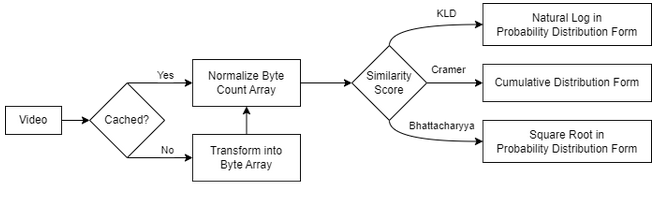
\includegraphics[width=\textwidth]{4 Design/4.3 Preprocess Data Flow.png}
    \caption{Pre-process Data Flow}
    \label{fig:preprocess-data-flow}
\end{figure}

To compute multiple similarity scores using homomorphic encryption, separate byte arrays are encrypted for each score. The recipient can perform computations with plaintext decimal values against the corresponding encrypted element in the array. This approach leverages the unique ability of fully homomorphic encryption and was borrowed from Pop-Share, as this approach is much faster than comparing ciphertext against ciphertext. 

For Kullback-Leibler Divergence, we share the PDF and its natural log. For each encrypted double in the PDF, we subtract the natural log of the plaintext element and multiply the difference. The product remains encrypted and is returned to the originator, where it can be decrypted. The summation is the similarity score.

For Bhattacharyya Coefficient, we share the square root of the PDF. For each encrypted double, we multiply the ciphertext by the square root of the plaintext element. The product remains encrypted and is returned to the originator, where it can be decrypted. The summation is the similarity score.

For Cramer Distance, we share the Cumulative Distribution Form (CDF) from PDF. The CDF is the cumulative sum of all of the elements in the PDF, such that the last value of CDF is equal to 1. For each encrypted double, we square the difference of the plaintext element. The product remains encrypted and returned to the originator, where it can be decrypted, and the square root of the summation is the similarity score.

In order to share the encrypted byte-count arrays, GhostPeerShare packages all ciphertext objects into an archive. The encrypted parameters and any associated data are stored as binary files, with each algorithm (e.g., $kld\_logX$) using 60 binary files, each representing one second of a one-minute video. This structure is particularly helpful for cases where video lengths differ, as it simplifies the trimming process. The binary files are then archived into an \textit{.enc} file format, which is unique to our application and contains both the encrypted data and a metadata JSON file with relevant video details (e.g., timestamp, length, frames per second). The archive averages around 40 MB on Linux for 1 minute of video.

\begin{figure}[t]
    \centering
    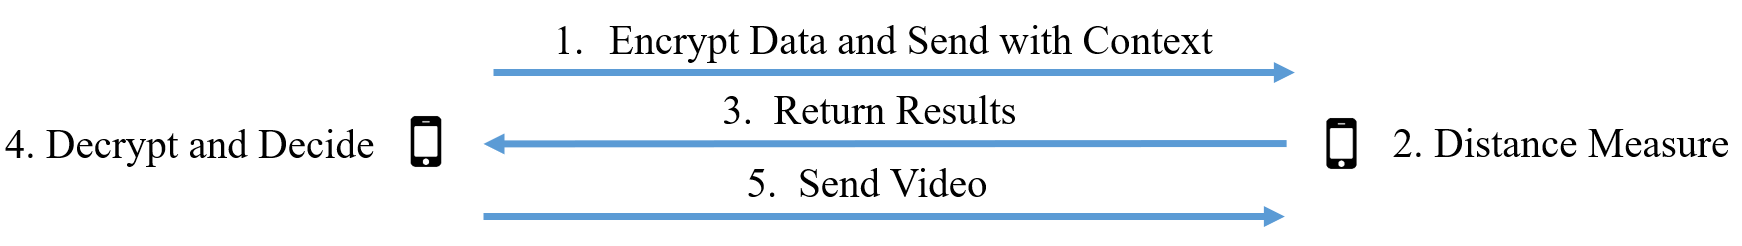
\includegraphics[width=\textwidth]{4 Design/4.3 Peer-to-Peer.png}
    \caption{Peer-to-peer Data Flow}
    \label{fig:peer-to-peer-data-flow}
\end{figure}

To facilitate a peer-to-peer exchange of files shown in Figure \ref{fig:peer-to-peer-data-flow}, GhostPeerShare supports QuickShare \cite{samsung_quick_2020} for Android devices. QuickShare [10] was developed by Samsung as a file-sharing utility application for nearby wireless devices. It leverages Bluetooth to discover nearby wireless devices and optionally uses WiFi to transfer large files between two nodes. QuickShare is accessible through a Flutter plugin that enables users to share data using their device’s native sharing capabilities. This allows each node to asynchronously send and receive files, leveraging a built-in Android feature rather than embedding similar functionality within the Flutter application.


% ========== Chapter 5

\chapter{Results}

In this section, we compare our implementation to the foundational contributions of SSO and PPVS. In order to evaluate the accuracy of Fully Homomorphic Encryption Library plugin in Dart, we measure the amount of noise generated during encrypted operations. Next, we compare our implementation of our distance measures using the original pre-processed video frames from SSO. Next, we compare the same video from various angles and determine the accuracy of our implementation. Next, we compare the distance measures for similar scenes against different scenes. Finally, we compare the performance across linux and android devices.

\section{Noise Accumulation}

When performing fully homomorphic operations, a small amount of noise is introduced that affects the accuracy of the decrypted distance measure. If too much noise is accumulated, the plaintext cannot be recovered. Figure 1a represents the baseline Mean Error from Pop-Share, compared to our implementation in Table 5.1. For KLD, our implementation introduced twice the amount of noise than the original. For Cramer Distance, our implementation introduced half of the amount of noise than the original. For Bhattacharyya Coefficient, our implementation introduced half of the amount of noise than the original.

% \usepackage{amsmath}
% \usepackage{graphicx}
% \usepackage{array}

% TODO: 

\begin{table}[h!]
\centering
\begin{tabular}{|c|c|c|}
\hline
\textbf{Function} & \textbf{Pop-Share} & \textbf{GhostPeerShare} \\
\hline
KLD     & $4 \times 10^{-9}$ & $1.78 \times 10^{-6}$ \\
Cramer  & $8 \times 10^{-4}$ & $6.54 \times 10^{-10}$ \\
BC      & $1.3 \times 10^{-1}$ & $6.34 \times 10^{-10}$ \\
\hline
\end{tabular}
\caption{Comparison of Mean Errors for Different Functions}
\end{table}


foobar

% ========== Chapter 6

\chapter{Discussion}

\section{Limitations}
\section{Qualitative Analysis}

%
% ==========   Bibliography
%
\nocite{*}   % include everything in the uwthesis.bib file
\bibliographystyle{plain}
\bibliography{uwthesis}
%
% ==========   Appendices
%
\appendix
\raggedbottom\sloppy
 
% ========== Appendix A
 
\chapter{Where to find the files}
 
The uwthesis class file, {\tt uwthesis.cls}, contains the parameter settings,
macro definitions, and other \TeX nical commands which
allow \LaTeX\ to format a thesis.  
The source to
the document you are reading, {\tt uwthesis.tex},
contains many formatting examples
which you may find useful.
The bibliography database, {\tt uwthesis.bib}, contains instructions
to BibTeX to create and format the bibliography.
You can find the latest of these files on:

\begin{itemize}
\item My page.
\begin{description}
\item[] \verb%https://staff.washington.edu/fox/tex/thesis.shtml%
\end{description}

\item CTAN
\begin{description}
\item[]  \verb%http://tug.ctan.org/tex-archive/macros/latex/contrib/uwthesis/%
\item[]  (not always as up-to-date as my site)
\end{description}

\end{itemize}

\vita{Jim Fox is a Software Engineer with IT Infrastructure Division at the University of Washington.
His duties do not include maintaining this package.  That is rather
an avocation which he enjoys as time and circumstance allow.

He welcomes your comments to {\tt fox@uw.edu}.
}


\end{document}
